\chapter{User Manual}

It is easy to get start using Buffalo. I assume you are reasonably familiar with the Visual Studio IDE and the general layout of the solution structures. I also assume you know how to compile a solution and where to find the compiled assembly. Since Buffalo is developed in VS2012, it is recommended you have similar IDE installed.

\section{Compiling}
To begin, first download the full source code from https://github.com/wliao008/buffalo. Open buffalo.sln in VS2012 and compile the source code. This will produce the Buffalo.dll and BuffaloAOP.exe in their respective bin/debug folder. We are ready to begin using it.

\section{Simple Profiler}
In this example we will create a profiler for our application. Suppose we have the following simple program.

\begin{lstlisting}[caption={Hello program}, label=helloprogram, frame=tb, basicstyle=\scriptsize]
using System;

namespace Hello
{
    class Program
    {
        static void Main(string[] args)
        {
            Hello h = new Hello();
            h.SayHello();
            h.Say("Hey Buffalo how's it going!");

            //pause the console
            Console.Read();
        }
    }

    public class Hello
    {
        public void SayHello()
        {
            Console.WriteLine("Hello World!");
        }

        public void Say(string msg)
        {
            Console.WriteLine(msg);
        }
    }
}
\end{lstlisting}

When the program runs, it will display the following:
\begin{lstlisting}[caption={Hello program output}, label=helloout, frame=tb, basicstyle=\scriptsize]
Hello World!
Hey Buffalo how's it going!
\end{lstlisting}

If we want to monitor the program, we can easily create a aspect to do the work.

\begin{lstlisting}[caption={TraceAspect}, label=traceaspect, frame=tb, basicstyle=\scriptsize]
using Buffalo;
using System;

public class TraceAspect : MethodBoundaryAspect
{
    public override void Before(MethodArgs args)
    {
        Display("ENTERING", args);
    }

    public override void After(MethodArgs args)
    {
        Display("EXITING", args);
    }

    public override void Success(MethodArgs args)
    {
        Display("SUCCESSFULLY EXECUTED", args);
    }

    public override void Exception(MethodArgs args)
    {
        Display("EXCEPTION ON", args);
    }

    void Display(string title, MethodArgs args)
    {
        Console.WriteLine("{0} {1}", title, args.FullName);
        foreach (var p in args.Parameters)
        {
            Console.WriteLine("\t{0} ({1}) = {2}", p.Name, p.Type, p.Value);
        }
    }
}
\end{lstlisting}

We can apply this aspect in three different level, lets apply it to the Hello class for example.
\begin{lstlisting}[caption={Apply Aspect to the Hello Class}, label=helloaspect, frame=tb, basicstyle=\scriptsize]
[TraceAspect]
public class Hello
{
	//...
}
\end{lstlisting}

With the aspect in place we can now invoke the BuffaloAOP.exe to perform the weaving. First, copy Buffalo.dll, BuffaloAOP.exe and Mono.Cecil.dll to a separate folder, lets call it the Buffalo folder.

Open a command prompt, navigate to the above Buffalo folder. And issue this command:
\begin{lstlisting}[caption={Invoking BuffaloAOP.exe}, label=buffalocmd, frame=tb, basicstyle=\scriptsize]
C:\Buffalo>BuffaloAOP.exe <path to the hello program exe>
\end{lstlisting}

Where you will supply the complete path to the hello program's assembly. If everything goes well BuffaloAOP.exe will perform the injection and put the final assembly in the Modified folder inside the folder of the target assembly. Now when the program runs, it will display the following output:

\begin{lstlisting}[caption={TraceAspect output}, label=traceaspectout, frame=tb, basicstyle=\scriptsize]
ENTERING System.Void Hello.Program::Main(System.String[])
        args (System.String[]) = System.String[]
ENTERING System.Void Hello.Hello::.ctor()
SUCCESSFULLY EXECUTED System.Void Hello.Hello::.ctor()
EXITING System.Void Hello.Hello::.ctor()
ENTERING System.Void Hello.Hello::SayHello()
Hello World!
SUCCESSFULLY EXECUTED System.Void Hello.Hello::SayHello()
EXITING System.Void Hello.Hello::SayHello()
ENTERING System.Void Hello.Hello::Say(System.String)
        msg (System.String) = Hey Buffalo how's it going!
Hey Buffalo how's it going!
SUCCESSFULLY EXECUTED System.Void Hello.Hello::Say(System.String)
        msg (System.String) = Hey Buffalo how's it going!
EXITING System.Void Hello.Hello::Say(System.String)
        msg (System.String) = Hey Buffalo how's it going!
\end{lstlisting}

Line 7 and 12 are the original method output, the rest are the output of the various interception points. Note that line 11 also capture the parameter value passed into each method and is available from the aspect.

\section{Hooking Up With Microsoft Build System}

Beside running from the command line, Buffalo can be hooked up with MS-Build, so post compilation weaving can be invoked automatically. Note that the instruction provided here are just the bare bond to get Buffalo going, a lot of bell and whistle are omitted here.

MS-Build is integrated with Visual Studio IDE via configuration file. For example, a C\# project has the associated .csproj, if open in a text editor you will see a line that reference a different configuration file: Microsoft.CSharp.targets. This file in term reference Microsoft.Common.targets.

Each .NET version has a Microsoft.Common.targets file. Depending on the version you are using, open up this file in a text editor. For example, for .NET 4.0, this file is located in C:\textbackslash Windows\textbackslash Microsoft.NET\textbackslash Framework\textbackslash v4.0.30319\textbackslash Microsoft.Common.targets.

Under the Compile section, add the line to import the Buffalo.targets file as shown in figure~\ref{buffalo_targets}

\begin{figure}[H]
  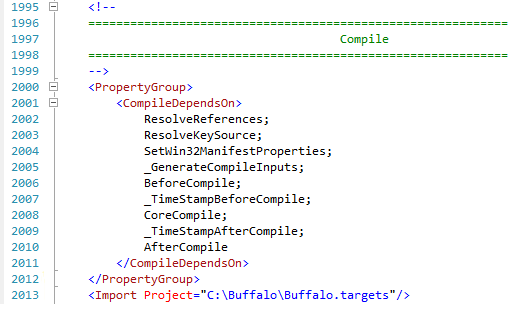
\includegraphics[scale=1.0]{CommonTarget.PNG}
  \centering
  \caption{Adding Buffalo.targets\label{buffalo_targets}}
\end{figure}

Create a folder and put BuffaloAOP.exe, Buffalo.dll, Mono.Cecil.dll in it, you can also put the config file Buffalo.targets (found in the client project) here. Modify the above to point to Buffalo.targets.

Open Buffalo.targets in a text editor. For the Exec Command, modify the path to point to the folder created above.

This is it. Now every time a C\# project is compiled, Buffalo will be invoked automatically.
